
 
% \section{ADVICE Paradigm}
% CROWDEDN where N=0-4 versions will be developed iteratively to help evaluate each version formatively and summatively.

% % \subsection{CROWDED1 -- Multiple Stakeholder knowledge}
% % The design of CROWDED1 will be motivated by the cues discovered using CROWDED0 during our empirical investigations. Cues are the cognitive and social weights for the model. Based on our findings, we will create a proof-of-concept CROWDED1 for allowing decision making. 

% % \subsection{CROWDED2 -- Cloud Knowledge}
% % CROWDED2, the cues for cloud knowledge (Table 2 will be collected using automatically using a crawler as in our previous studies. The model weights will populate based on model evaluation of cues and fine-tuning them. 

% \subsection{CROWD3 -- Verification}

% % One limitation of the CROWDED 0-2 is that it accept all advice, uncritically. However, humans have fixed and limited attention spans~\cite{davenport2001attention}  which they  have learned to hoard and use sparingly.  
% % Hence, humans  use heuristic ``short cuts'' that let 
% % them satisfy the demands of their work, just enough, before rushing off to their next
% % task~\cite{simon1956rational}.
% % Such heuristics are essential if humans are to tackle their busy workloads but
% % can lead to faulty advice. Hence we must ask:

% We plan to adapt methods from the qualitative and quantitative
% literature for automatically generating the fixes, then presented to our stakeholders.



 





\section{Methods }\label{rqs}
Recall from our introduction that we have three kinds of  experiments.   In our
\underline{\bf CPU-intensive studies},
\IT~ will explore the requirements to find the most interesting/dangerous scenarios within the requirements space. We anticipate running millions of   CPU-intensive studies.

In our
\underline{\bf human-intensive studies}, we will test if teams share the same vision of the requirements.  Here, teams will  
play a simulation game where they must monitor a fleet of drones, watching for behavior that violates the requirements.
Unbeknownst to them, the game will then enact the danger scenarios found
in the CPU-intensive studies.    We anticipate running a few hundred human-intensive studies.

Finally, we will  also run   \underline{\bf ablation studies} where   dangerous scenarios must be handled by (a) the AIs without human input or (b) the humans without AI input



\subsection{Participants}
\noindent
 \IT~  is a team-based human-in-the-loop AI optimizer and so to assess this tool, it must interact with teams of either (a)~humans or 
 (b)~human surrogates. 

Initially, small student studies  (run with by NC State students) will be conducted to evaluate  \IT. 
Subsequently, we will recruit subject matter experts from the SMART-STEReO team.

As to the surrogates, for CPU-intensive studies will need some oracle that can offer opinions which \IT~ can use to prune the search space. These surrogates will be built automatically using data miners applied to the   electronic footprint (see Table~\ref{info}).






\subsection{Interface}\label{interfaces}
\noindent

This research will explore  CPU-intensive studies and human-intensive studies.
In the CPU-intensive studies, humans will occasionally be asked a few questions
by \IT. For this kind of study, humans will interact with \IT~ via a simple chat bot that will share text questions, perhaps sometimes a small histogram showing the effect of different choices of domain data distributions.

\begin{wrapfigure}{r}{2.5in}
\includegraphics[width=2.5in]{fig/ewpmt.jpg}
\end{wrapfigure}
For other kinds of human-intensive studies, we will build a game where teams watch over a fleet of drones.
In that game, the screen will show a interactive topological map:
\bi 
\item    Markers will indicate locations  of   drones and humans.
\item Mousing on a region  will pop up   details on that region.
\item Mousing on drones will let humans     control the drones.
\item
Occasionally, little alert flags will pop-up pointing out potential pitfalls in the current situation. Each alert will come with a set of succinct questions offering suggestions on how to manage that alert,
plus one more option called ``other'' that will let operators do anything they like. Those alerts, including the suggestions,  will  be generated by our swarm optimizers running in the background, advising of events/decision that have  a high probability of making things better/worse. 
\ei
That interface will be iteratively improved based on evaluation from multiple stakeholders of various expertise (student novices and professionals) and genders. Co-PI Kuttal has created human-centric tools for developers using user-centered design and evaluation approaches.  
Previously, she has created tools that support programmer creativity \cite{Kuttal2020} and exploratory programming behavior \cite{Jernigan2017, Jernigan2015}, debugging web-based distributed programming \cite{KuttalSR13-chi, KuttalSBRKS19}, % REMOVED: KuttalSR13
problem-solving techniques \cite{Jernigan2017, Jernigan2015}, gender-specific behavior \cite{Kuttal2021g, Kuttal2019, Alexposter2022}, socio-technical skills \cite{Abimposter2022,Abimgitposter2022,Diwanjiposter2022,Zhou2018, sarma2016hiring, KuttalCWBS21, KuttalSRW18, abs-1810-13062} and communication styles \cite{Kuttal2020}.



 
\begin{table}[!t]
\caption{ In M-of-N studies,  a few $M$ humans monitor a large number of $N$ drones. }\label{mns}
{\small
\begin{tabular}{|p{.98\linewidth}|}\hline
\rowcolor{blue!10}
In an  {\em  m-of-n} study,  teams of $M$ humans will play a simulation game in which they must 
 monitor a fleet of   $N$ drones,   watching for off-nominal
situations, intervening when necessary.  \\
Just to give a flavor of the off-nominal problems our humans might be asked
to manage, here a few examples:
\bi
\item An emergency  team laying down a back burn must have a workable escape route.
Hence, if that team is working at one end of road and,   several miles away, a brush fire is encroaching   the escape route, then we must intervene to order the crews to down tools and rush their escape.
\item 
Drones in urban areas can fly up to 400' while Cessnas, monitoring those drones,
can fly down to 500'. In the case of approaching high winds, we must intervene to order the Cessnas to fly higher. \ei\\
\rowcolor{blue!10}
Note the monitoring challenge of the above two examples. Firstly, to see the problem, humans have to synthesize connections between
events occurring in remote parts of the simulation game.
Secondly, each drone in isolation could be working perfectly.
But when sets of drones co-ordinate with humans in a shared
space, some problems (like those above) become emergent.\\\hline
\end{tabular}}
\end{table}

\subsection{User Studies}
\noindent
Table~\ref{mns} discusses  the   ``m-of-n-studies''  used for our human-intensive studies. In these studies, a small number of human watch over a large number of drones looking for requirements violation.
\mbox{M-of-n studies}  are an excellent tool for controlled experimentation since they can  be run under a variety of well-controlled variations; e.g.
\bi
\item 
Decrease team size $M$; increase
number of drones being monitored $N$; 
\item 
Increase the number of problems introduced; 
\item 
Decrease the time available for solution etc.\ei 
% These times required to humans to detect, then respond, to requirements violations within the simulation
% can  be {\bf ablation studies} (see out text). \ITS{1} will be a success if the reaction times are faster and the proposed response is better when humans and AI work together to create those responses.
For the participants of such m-of-n studies, the challenge is staying alert   while   monitoring
all the information coming in from a large fleet of drones (visual images, sensor readings of the environment
inside and outside the drones, wind and weather reports, positions of humans on the ground, etc).
Faced with this information overload,
human operators often  become bored and fatigued and  distracted and   slow to recongize and react to new problems.  
 

 We conjecture that \IT~can address   operator fatigue.
 Rather than asking humans to watch all instruments reporting all features of model,
 we could ask instead for humans to engage with 
\IT.   \IT~ is a tool
 for ignoring most of the data and focusing instead on just a small region.
 We conjecture that by  
 tuning
the   frequency at which \IT~ interacts with humans, we think it possible
that can   engage the humans in some interesting, but not very taxing, problem
solving. If we tune correctly, then
these alerts will engage, not exhaust, the humans and so,  when novel and dangerous situations arise, humans
will quickly recognize and respond.

For further details on our user studies, see Table~\ref{studies}.




% All our studies   will cycle through two phases:
%  \bi 
%  \item For three cycles (run on different days):
%  \bi 
%  \item In the  \underline{\bf experience} phase, teams of participants   interact with the current requirements (with out without \ITS{1}) 
%  for a range of case studies for one to three hours. 
%  \item In the \underline{\bf debrief} phase, team members will debate why  they made different decisions about similar scenarios.
% We expect the debrief stage will lead to an update in the  requirements plus    updates to the control parameters of a model.
% A subsequent {\bf experience} phase will then test those updates.
% \ei
% \ei
% With the exception of some of the ablation studies (discussed below),
% \ITS{1} can be potentially beneficial  in both the {\bf experience} phase and {\bf   debrief} phase.
% During   the {\bf debrief}, \ITS{1} will help humans explore  trade-offs within a large space
%  of requirements.
%  Also, during the {\bf experience} phase, \ITS{1}  could    focus the human's attention on just the most important parts of the data

 


 

\begin{table}[!t]
\caption{Notes on our human-intensive studies.}\label{studies}
{\small
\begin{tabular}{|p{.98\linewidth}|}\hline 
\rowcolor{blue!10}
User studies will be conducted after the approval for
 NC State Investigator Review
Board (IRB). \\ 

We will match   user studies to the participant skills.
  Simple user studies (e.g. Amazon drones delivering packages to households, during
a thunderstorm) will be used for our work with NC State students.
On the other hand, 
the fmdtools models of \S\ref{egmodel} will be used in association with subject matter experts from the SMART-STEReO team. 
\\\rowcolor{blue!10}
Initially, we will work with teams of size $N=2$, then move to larger teams for years two and three.\\
Initially, we will run   simple user studies (e.g.a fleet of drones  delivering Amazon packages during a thunderstorm)
then  move to move complex studies. Finally, in year 3 we will explore  
{\bf case studies} based on the emergency response teams modeled in the fmdtool models generated
by the SMART-STEReO team.
\\\rowcolor{blue!10}
For our  initial small \underline{\em lab studies}
we will recruit university students. \\\rowcolor{blue!10}
For our \underline{\em case studies}, we will recruit  real-world subject matter
experts from the SMART-STERe team.
\\
 All our lab studies and case studies will explore models at various levels of ``stress''.
Stressing factors could be ``achieve more goals with fewer drones''; ``achieve more goals in less time'';
``achieve more goals with fewer team members'';
``achieve more goals in the presence of an increasing number of non-nominal scenariois'';
``achieve more goals when the time-to=failure of each drone becomes increasingly variable''.   \\\rowcolor{blue!10}
For data collection in these lab studies and case studies, we will:
\bi 
\item Initially use a
  think-aloud protocol \cite{lewisusing, Seaman1999} 
  where participants will   vocalize their thoughts and feelings as they perform their tasks.
  \item Conduct retrospective interviews to gain insights into participant experiences and barriers encountered during decision making with and without {\IT}.
  \item At the end, we will measure the cognitive load of the humans and usability of {\IT}. \ei \\
As in our past qualitative analyses (e.g., \cite{Kuttal2020, Kuttal2021g}), we will triangulate (compare and attempt to refute) the results with interviews and surveys to understand their strengths. %Retrospective interviews will be conducted to gain insights into participants' experiences and barriers encountered during decision-making with and without {\IT}. 
We will collect (1) Pre-surveys with standard questionnaires to collect demographics and familiarity with the domain of the model. (2) Pre- and post-surveys with standard questionnaires will be used to evaluate self-efficacy. (3)  User Experience Questionnaire (UEQ)~\cite{rauschenberger2013efficient,schankin2022psychometric,schrepp2014applying} to evaluate the usability of  {\IT} interface. (4) Measure participant engagement with the {\IT} tool using the ISA engagement scale \cite{soane2012development}, which is based on the view that engagement comprises 'intellectual,' 'social,' and 'affective' dimensions. (5) Post-surveys will be used to analyze the cognitive load \cite{CognitiveLoad}(such as using NASA Task Load Index~\cite{hart2006nasa})  to measure and conduct a subjective mental workload (MWL) assessment. \\\hline
\end{tabular}}
\end{table}

% For starters, we need to implement the PSO and LLM extensions described above. In our experience, this will raise numerous   design questions about the relative metrics of some tactic versus another;
% e.g.
% \bi 
% \item 
% Currently \ITS{0} clusters over some synthesized dimension that is analogous to PCA; so
% should \ITS{1} do that, or employ some other clustering method?
% \item Peng et al.~\cite{peng2022godel} assert that mixing gold plus rusty quries is useful for building LLM training sets.
% But does that policy work in this domain?
% \ei 
% The merits of these different tactics will have to be assessed with respect to case studies with real models and real subject matter experts.


\subsection{Measurements}
{\noindent}Table~\ref{metrics} shows the   independent and dependent variables to be collected as part of this study.  Most of these measures are self-explanatory; e.g. whatever we do with \IT~  and human-in-the-loop reasoning, we need to benchmark that against state-of-the-art fully automatic optimization tools such as FLASH, HYPEROPT and OPTUNA~\cite{bergstra2015hyperopt,nair18,akiba2019optuna} (see Table~\ref{metrics}, bottom-right, ``{\em nonhuman y-metrics}'').

But there are two sets of metrics worthy of discussion. Recall from the above that stakeholders are assigned their own particles which move from some initial
position to some final position. By measuring the median difference in particles between different
stakeholders before and after inference, then we can report initial and final divergence in team 
 opinion (and {\em decreased} divergence would be {\em better}). This metric is shown bottom-right of Table~\ref{metrics}
 as ``Initial and final divergence''.

 Also of note is the ``{\em cognitive load on the humans}'' shown top-right. Within the  cognitive psychology literature,
 there is a standard   questionnaire~\cite{CognitiveLoad} to quantitatively gauge cognitive load.


 


% Note the requirements engineering aspects of these m-of-n studies:
% \bi 
% \item To recognize ``off-nominal'', team members must have a shared understanding of what requirements need to be followed.
% \item To ``intervene when necessary'', team members must understand the capabilities of their tools such that they know what to adjust to repair   off-nominal events.
% \ei 


 

%%%%Recall from the above that stakeholders are assigned their own particles which move from some initial
% position to some final position. By measuring the median difference in particles between different
% stakeholders before and after inference, then we can report initial and final divergence in stakeholder
% opinion.
 


% in some analogue of PCA
% One factor that greatly simplifies all this experiemtnal work 

% Initially, small \underline{\em lab studies} will be conducted to understand developers' decisions in controlled environments. We will work with teams of size $N=1$, then move to larger teams for years two and three.

% After these smaller scale lab studies will come much larger scale
% \underline{\em case studies}.  For our \underline{\em lab studies}
% we will use university students   and for our \underline{\em case studies}, we will
% use teams use participants from the teams writing the models of \S\ref{egmodel}.
% Note that Co-PI Kuttal is  particularly skilled   with such lab studies and case studies (e.g., ~\cite{Kuttal2019, Lott2021}).

 
% \begin{wraptable}{r}{2.25in}
% \footnotesize
% \centering
% \caption{i* Models from~\cite{mathew2017shorter}.}
% \begin{tabular}{r|rr }
%  \textbf{Model} & \textbf{Nodes} & \textbf{Edges}     \\ \hline
% Services, see Figure~\ref{fig:scrumModel}.  & 351 & 510    \\
% Counselling & 350 & 470    \\
% Marketing & 326 & 422   \\
% Management & 206 & 239    \\
% ITDepartment & 126 & 162    \\
% Kids\&Youth & 81 & 81      \\
% IT Modernization & 53 & 57    \\
% \end{tabular}
% \label{tab:sizes}
% \end{wraptable}
%  \underline{\bf TASKS:}
%  As stated in the introduction,
%  we will run three studies. 
% A common feature 


% To avoid those problems, \ITS{1} will simulate models
% of the  emergency services' requirements. 
% In {\em CPU-intensive studies},  \ITS{1} will explore the requirements to find the most interesting/dangerous regions of the problems space. 
% Also, in {\em human-intensive studies}, we will see how early humans can detect and repair off-nominal drone behavior.  Humans will be asked to play a simulation game where they must monitor a fleet of   drones,  intervening when necesary. Unbeknownst to them, the game will  enact the   danger
% scenarios found in the CPU-intensive studies. 
% The \ITS{1} human-in-loop optimizer will be judged a success if, in the CPU-studies, it can quickly find the most interesting/dangerous scenarios. Further, in the human-intensive studies, success means that \ITS{1}'s questions   keeps the stakeholder engaged (but not exhausted) such that,  when danger scenarios creep in, they can quickly detect and mitigate them.

% Further, to test the above conjecture, we would then run an {\em ablation study} where the danger scenarios must be handled by (1)~the AIs  without human input or
% (2)~the humans without AI input.

 
% Our experiments will focus on \underline{\em serial  RE discussions} where some design artifact (the model) is being passed along a circle of stakeholders who may update the model before passing it down the circle
% (stopping when the model
% traverses the entire circle
% without revisions or comments).


% (Aside: For future work, we will explore ``parallel RE design discussions'' where N people
% debate the same version of a model at the same time (e.g. at some meeting). In justification of this focus on serial distributions, we note that this is a natural model for geographically remote workers who usually work on by themselves, sometimes interrupted by messages, emails, or status meetings with their manager.)


% In this work, we will also   explore gender issues leading to biases   using GenderMag \cite{Guizani, Chatterjee}, to  find and fix gender-related issues in problem-solving   and increase gender inclusiveness. 



 % \underline{\bf   INTERFACE:}
 % To begin with, our bot will offer a very simple text interface, sometimes with a question "rank the following
 % two options".  
% Initially, we will offer our participants
% a DISCORD channel to handle (and record) design discussions
% plus a 
% a simple directed-graph editor (with a search bar) to view our models. Edits to the model will be saved as pull-requests within Github (thereby offering a record of all revisions to model, tagged with the name of the person proposing a change.


% The final version or deployment version will be provided with a more sophisticated interface that allows explaining the decisions of the ADVICE. Further, it will also give suggestions based on the
% electrong footpring and teams during the decision-making process of stakeholders. The explanation and suggestions  will follow Shneiderman's guidelines \cite{Shneiderman1982} and Neilsen's heuristics  \cite{Nielsen1990}. 

%  \underline{\bf   CASE STUDY MATERIAL:}
% The first step in the workflow is to gather the requirements con-ops documents from different emergency response teams, then build their associated fmdTools models. This first step has been underway now for two years and this proposal will take advantage of that work product. 

% Next we will script up the environment that can run the fmdTools models, and display their results. Some visuals will be added to observes can imagine that this data is collected from  
 
%  After that, we will have meetings with the SMART-STEReO team to identify some useful scenarios (perhaps, even, looking at their historical logs to see what kinds of simulation results lead to most changes
%  to their models). 
%  The scoped studies will then be sorted by ``domain knowledge needed to monitor the drones''.
%  If the domain knowledge is something simple like ``do not run out of fuel'' or ``do not exceed this threshold for max acceleration'', the scenarios are suitable candidates form our studies with NC State students. And if the required domain knowledge is complex such as ``implement standard operating procedures for firefighters in a class7 smoke-field envrionment'', then that scenarios would be slated for running with volunteers from the SMART-STEReO team.

% At that point we can start the CPU-intensive studies to find the most severe problems with the current requirements.  Once found, we would cache those problem scenarios (for use in the human-intensive studies) before asking the CPU-intensive studies
% to search for mitigations to those problems.

% Once we have some interesting problems, we can start the human-intensive studies.

 
 

%   \underline{\bf CASE STUDY MATERIAL:} Year1 (with NC State students) will use 
% relatively simple models taken from the SE research literature (e.g. the product line of Figure~\ref{fig:scrumModel}. Then, to stress test our ideas,  we would take advantage of the flurry activity around the SMART-STEReO group building the \S\ref{egmodel}'s models. As mentioned above, this is a very active and well-funded group doing much current work.  We would watch that activity, find decisions are made based on simulation output, and then \underline{{\bf replay those decisions}} with our tools (to see if a different and better conclusion might be reached, using less simulation time). 
  
% \underline{{\bf Replaying those decisions}}  will not be an onerous task.
% Firstly,  the SMART-STEReO group has an established procedure for sharing models.   In the COVID era, to enable remote work on that project,
% this group created policies by which they can build laptop software with all the licenses and permissions needed to work securely on these materials. Now it is routine for that group
% to have interns working on those models, from around the country, logging-in via those secure laptops.

% Secondly, repeating a simulation study is often a daunting task, since it requires the CPU farms needed for the original study. But recall that {\ITS{1}} uses
% {\ITS{1}} recursive bi-clustering procedure, evaluating only 2 examples at each level of the recursion\footnote{Formally, this makes {\ITS{0}} akin to the SIMPLEX method~\cite{muller1979location} that finds vertices
% of a system of linear inequalities,  then favors samples of those points (since they
% are most informative). \ITS{0}  searches through some data points that fall within some multi-dimensional polyhedron. \ITS{0}'s search for distant points means that  it finds, then evaluates, the vertices of that polyhedron-- which is a non-parametric analogue to the  points sampled via   SIMPLEX. But note that we favor \ITS{0}'s method over SIMPLEX since the latter requires optimization problems expressed in some high-level equational form (whereas \ITS{0} can work
% from the log of the output of any model at all).}. In practice, this means that {\ITS{0}} (and hence {\ITS{1}}) should be able to replay
% conclusions from $N$ evaluations using just  $2\log_2{(N)}$ evaluations
% Better yet, we may not even have to rerun the simulations.
% With access to a log of all the evaluations made during the original study, we might be able to use some partial match approach to make do with similary, but not exact, old rows for our new queries.


  

 

%This workflow will  make it convenient to conduct large scale studies where we invite (say) 1000s of industrial practitioners (via email) in order to attract 100s of participants.






%   Some of our research questions (see below) require us to run numerous large teams.  For that purpose,
% we will use Mechanical Turk (MTurk) to recruit  large sets of participants (>300). MTurk is used extensively by academics as a quick and cheap means of collecting questionnaire data, including software engineering research, from a diverse sample of participants.  E.g. Stolee used "Turkers"   look for bugs in regular expressions~\cite{stolee2010exploring} while Stolee and Menzies
% used "Turkers"  to comment on Github pull requests~\cite{chen2019replication}.
% When using MTurk it is important to 
%   augment any pre-screening with "gold tasks"
% which are a small number of work packets with known results that are slipped into
% the "Turkers" workflow. By pruning "Turkers"
% who fail on the gold tasks,  Stolee and co-PI Menzies found   that at least  50\% of
% their workers has sufficient skills relevant for details SE design and implementation tasks.

% Initially, we will   balance gender and race since prior studies warn that  such balance  is crucial to prevent algorithms from perpetuating social inequities~\cite{Leavy2018}.
% Later,  when \ITS{4}   explore issues of bias and discrimination, we will use teams with a   variety of diversities.
%  We will conduct multiple lab studies to bolster confidence in the results. To allow more gender and expert diversity we will conduct virtual lab studies.  Virtual lab studies will recruit participants via snowball sampling, ads on social platforms, and recruitment websites such as Upwork.



 


% Furthermore, since the literature \cite{Kuttal2019, Lott2021} indicates gender differences in communication, more comprehensive gender-inclusive language  \cite{festante2007, miller2001handbook} is needed to prepare suggestions to engage, provide non-authoritative suggestions \cite{Seymour2017}. In order to generate accurate suggestions, we may need to consider cues from both study participants as well as cloud. 

 % \underline{\bf METHODOLOGY:} 

 % XXX? i
 
% For data collection,
% the think-aloud method \cite{lewisusing, Seaman1999} will be used. Participants will   vocalize their thoughts and feelings as they perform their tasks.   Participants in a control group will perform tasks using appropriate state-of-the-art optimizers suitable for comparison with automated version of {\IT}. Based on our literature review~\cite{lustosa21} (as of 2021) FLASH and HYPEROPT and OPTUNA~\cite{bergstra2015hyperopt,nair18,akiba2019optuna} will be utilized
% (we will update those comparison
% tools to reflect the ongoing state-of-the-art).

% As in our past qualitative analyses (e.g., \cite{Kuttal2020, Kuttal2021g}), we will triangulate (compare and attempt to refute) the results with interviews and surveys to understand their strengths. Retrospective interviews will be conducted to gain insights into participants' experiences and barriers encountered during decision-making with and without {\IT}. We will collect (1) Pre-surveys with standard questionnaires to collect demographics and familiarity with the domain of the model. (2) Pre- and post-surveys with standard questionnaires will be used to evaluate self-efficacy. (3) Post-surveys will be used to analyze the cognitive load using NASA Task Load Index~\cite{hart2006nasa}  to measure and conduct a subjective mental workload (MWL) assessment. 
 

 
%  \underline{\bf DATA ANALYSIS:} Our specific research questions require the collection of specific metrics:
% \bi
% %  Video data, audio data, and screen interactions of developers will be collected as transcripts, which will be analyzed using a mix of qualitative and quantitative measures. Qualitative methods from Grounded Theory \cite{GlaStr67} (e.g., Corbin and Strauss variant \cite{strauss1990basics}) will be used to analyze the transcripts.  We will annotate points based on developer utterances to identify key concepts and phenomena via an iterative, open-coding process, especially for artifacts or experience-based cues when making decisions.  This process will also be used to analyze decision-making behavior.   Finally, thematic analysis \cite{Braun2006} will be used to organize qualitative data into themes that relate back to the research questions.  Non-parametric effect size and significance tests   will be used for quantitative analysis.
% % Further to the above, some of 
% \item
% \underline{\em Stakeholder category metrics :} One goal of this work is to better support model-based reasoning for different categories.
% Under some anonymization   protocol, {\em participant diversity} will be collected
% (with categories such as age, gender, racial background, veteran status, accessible challenges, etc.)
 
% % \underline{\em Bias Metrics:} Our bias mitigation metrics
% % were discussed in \S\ref{bias}. Note that we would ensure we can report  these metrics separately
% % for all different stakeholder categories.
% \item
% \underline{\em Initial and final divergence metrics:} For   teams of size $N>1$, we   use PSO to measure initial and final divergence before and after   inference 
% (and, ideally, that difference decreases from initial to final).
% Recall  from the above that   stakeholders
% are assigned their own particles which
% move from some initial position to some final position. By measuring the median difference 
%  in particles between different stakeholders before and after inference, then we can report   
%  initial  and   final
%  divergence  in stakeholder opinion.
% \item
% \underline{\em   $y$ metrics:} Stakeholders  often explore
% multiple goals, where the $y$ goals might be contradictory. We need some trade-off predicate
% that knows how to report improvements on multiple dimensions. We will use the
% Equation\ref{eq:cdom}  calculation
% from Table~\ref{advice1}. As mentioned above,  this calculation is  preferred to  standard ``boolean domination'' (one thing is better than another if it is no worse on any criteria and better on at least one criterion), since it is known that boolean domination can  fail for three or more goals~\cite{Wagner:2007, Sayyad:2013}.
% \item
%  \underline{\em Acceptance  metrics:}    $y$ metrics    only comment on terms     in a model. Above and beyond that, we need    our post-surveys to capture   other concerns from stakeholders   about the acceptability of our final models.
%  \item
% \underline{\em  Nonhuman-$y$ metrics:}
% To calibrate and baseline the {\IT} $y$-metrics, we collect output $y$ values
% seen in     AI tools that make all the decisions themselves, with no human involvement
% (e.g. 
% FLASH, HYPEROPT and OPTUNA~\cite{bergstra2015hyperopt,nair18,akiba2019optuna}).
% \ei
% % \textbf{Methodology} Each student will complete decision task using the think-aloud method. They will record their decision making sessions. We will conduct surveys on their experiences, knowledge tests and end-of-term student course evaluations. Each professional will complete decision based HIT (Human Intelligence Task) using MTurk followed by surveys on their experiences with CROWDED. HIT will have attention checks. An attention check is a question designed to verify that the respondent is reading questions and responding with care. 


%  \underline{\bf ABLATION STUDIES:} 
% % \textbf{Data Analysis} Quantitative measures (such as ANOVA) will be used to analyze the scores on tasks, and self-reported surveys on decision making experiences. 


\section{ Research     Plan}\label{rqplan}
For full details of our research plan,  see  the {\em Collaboration Plan} supplemental document. In summary:
\bi 
\item In all years, NC State will be a frequent visitor to the SMART-STEReO team (in California).
All user studies will be designed with subject matter input from that site.
\item 
Also, in year1, NC State will build {\IT}, version 0.1 and gaming interface. 
\item 
Year2, will have  some initial, and limited,   interaction between subject matter experts and our tools.
\item
In year3, much data will be collected from a very large number of user studies, many of which will include studies with participants from the  SMART-STEReO  team.\ei
Also, in all years, we will explore  {\em  broadening participation in computing}.
One  of the benefits of  NSF funding is the opportunity to work on  broadening participating in computing (BPC).  Our BPC plans are discussed in \S\ref{bpc}.  BPC will be an ongoing task through-out the work.

%Table~\ref{tbl:plan} shows some planned milestones for this research work. 


\begin{table}[!t]
\caption{Metrics for this Study.}\label{metrics}
{\small \noindent\begin{tabular}{|R{.12\linewidth}|R{.34\linewidth}|R{.48\linewidth}|}\hline
 \rowcolor{blue!10} Notes & Independent variables  & Dependent  variables  \\\hline
Human-level measures & 
\bi 
\item Demographics about teams: size of teams; years of experience with each other; etc. 
 \item 
 Demographics about individuals: age, gender, racial background, veteran status, accessible challenges, years of experience with the case study being used; etc.
\ei
&
\bi 
\item Time to recognize a requirements violation in the simulation;
\item Time to resolve that violation;
\item Number of delayed actions per minute;
\item  Number of forgotten  actions per minute;
\item Number of interrupted actions per minute;
\item Average interruption time (seconds per minutes)
 \item Cognitive load on the human. \ei\\
 \rowcolor{blue!10}  Domain-specific measures 
 (different case studies may have    different domain-specific success
criteria). & 
For example:
\bi 
\item 
Types and size (number of words) of electronic footprint available  per team member.
\item 
Size of requirements models; e.g. number of variables; number of constraints; 
average constraints per variable; etc.
\item Nature of the goal space; e.g. how many objectives; how many objectives are conflicting; etc. 
\ei & For example:
\bi 
\item When delivering packages for Amazon, the goal might be 
{\em most} packages delivered in {\em least} time by {\em fewest} drones.
\item for emergency response groups fighting  a brush fire,
the goals might be 
{\em minimize} the property damage  during  simulation of a brush fire while
also 
{\em minimizing } the lives lost or injured during the simulation of the brush fire. \ei\\
Domain-general measures 
(these should apply to most case studies)
& Amount of ``stress'' in the simulation. Recall {\em m-of-n} studies
can be stressed in various ways such as decreasing the number of $N$ humans,
increasing the number of $N$ drones; decreasing the required response time; increasing the number of
problems injected into a simulation.
&
The following are goals for the multi-objective simulation.
\bi 
\item {\em  Minimizing} acceleration stress on the drone rotors ;
\item {\em Maximize}   battery reserves when drones return to base;

\item 
{\em Acceptance metrics}:Using
post-surveys,  capture   concerns from stakeholders about the acceptability of our final models.
\item 
{\em Nonhuman-y metrics}: To calibrate and baseline the ADVICE y-metrics, we collect output y values seen
in AI tools that make all the decisions themselves, with no human involvement (e.g. FLASH, HYPEROPT and OPTUNA~\cite{bergstra2015hyperopt,nair18,akiba2019optuna});
\item {\em Initial and final divergence metrics}:   Looking at PSO particles,
measure  
divergence between team members before and after inference (ideally,   difference decreases from initial to final).
\ei\\\hline
\end{tabular}}
\end{table}


%\newpage
 \section{ Research Questions}\label{quest}

 

% Please add the following required packages to your document preamble:
% \newcommand{\X}{\ding{52}}
% \begin{table}[!t]
% \caption{Research Plan.}\label{tbl:plan}
% \footnotesize
% \begin{center}
% \begin{tabular}{lp{5in}|l|l|l}
% Task && Y1 & Y2 & Y3 \\\hline
%  Setup & Build a baseline implementation of \ITS{1}, version 0.1  & \X & \\
%  Bot   & Build   baseline versions of the interface & \X & &\\
%  RQ0&   Do people and \ITS{} find different solutions for completing design tasks?    & \X & \X & \X \\
% RQ1&   Do humans using \ITS{} perform better than (a) humans, fully manually  (b) AND   AI tools   humans? & \X & \X & \X \\
% RQ2 & How to select terms for prompt engineering? & \X & \X & \\
% RQ3&   For \ITS{1}, how to weigh PSO’s cognitive versus social reasoning?                &   & \X &   \\
% RQ4&   Is  \ITS{1},’s team support “useful”?                                              &   & \X &   \\
% RQ5&   Is there a max “team size” threshold above which \ITS{1} would not be recommended? &   & \X &   \\
% RQ6&   Are different kinds of background knowledge most useful for \ITS{2}?                    &   & \X &   \\
% RQ7&   Do different categories of stakeholders need different support for their different cognitive styles?                                      &   &   & \X   \\
% RQ8&   (if time permits) Can {\IT} support test case generation?                                          &   &   & \X\\ 
% RQ9&  (if time permits)   Can {\IT} guide the creation of the model?                                          &   &   & \X\\\hline
%  Also   & Work on BPC (broadening participation in computing).                           & \X & \X & \X  
% \end{tabular}
% \end{center}
% \end{table}


\subsection{{\bf CPU-Intensive} Questions} These research questions will focus on the measuring and then improving the algorithmic performance of \IT.

{\bf RQ1 (Year 2)  {\em For \IT, how should we weight PSO's cognitive versus social reasoning?} }
   Recall that PSO determines the new velocity of a particle from the sum of a personnel's cognitive weight
    $\phi_p$ and the group social weight  $\phi_g$.
    The specific values for these weights in this work will be determined through experimentation, potentially learned via a self-adaptive scheme~\cite{harrison2018self}
or through configuration hyperparameter optimization~\cite{8469102}). Initially, we consider the advice from Pedersen~\cite{pedersen2010good}, who recommend  $\phi_p+\phi_g \approx 4$ (bearing in mind that distance weights are normalized between 0 and 1). 
\underline{ Relevant metrics:} The vpttrvy $\phi_p+\phi_g$ optimizes for both the 
  y-metrics and
the acceptance metrics of   Table~\ref{metrics}, bottom-right.
% \end{description}
% \vspace{-10mm}
% \begin{description}


{\bf RQ2: (Year 1,2) {\em How do we choose terms for prompt engineering?}} Recall that researchers in large language models (LLM), such as Peng et al.~\cite{peng2022godel}, emphasize the importance of carefully selecting training words for LLM prompt engineering. As discussed in Section \ref{cloud}, Peng et al. recommend achieving an equal balance of terms with the highest and lowest language model (LM) loss. While this recommendation was valuable in their domain, in the context of our research questions, we will conduct experiments with term selection.
 %Recall that LLM researchers like Peng et al.~\cite{peng2022godel} recommend the careful selection of training words for LLM prompt engineering. As discussed in \S\ref{cloud}, Peng et al. recommend an equal balance of terms  with  highest and lowest LM loss. That was useful in this domain but in this resaerch questions,  we would experiment with term selection. 
  \underline{Relevant metrics:} The right term selection results optimizes for  
the acceptance metrics (see Table~\ref{metrics}, bottom-right). 

\subsection{{Human-Intensive} Questions}
In addition to qualitative measurements obtained through the Think-Aloud Protocol, which involves having users verbalize their thoughts and experiences during interaction to provide insights into usability, engagement, and cognitive load, we will employ behavioral observations. Behavioral observations entail observing user behavior, hesitation, and decision-making patterns during tasks. To complement these qualitative methods, quantitative measurements will be applied to address following RQs focused on the overall performance and usability of the \IT~tool.

{\bf RQ3: (Year 1,2,3) {\em What are the key usability factors of the \IT~tool, and how do they impact user experience for first responders?}}
In controlled settings, we will assess the usability and engagement of the \IT~Tool with and without it. Additionally, we will conduct comparisons with earlier versions of the \IT~Tool to ensure continual improvement in usability and engagement with each iteration.
\underline{Relevant metrics:} UEQ responses, IST scale responses, Time to recognize a requirements violation in the simulation; Time to resolve that violation; Number of delayed actions per minute; Number of forgotten  actions per minute; Number of interrupted actions per minute; Average interruption time (seconds per minutes).

{\bf RQ4: (Year 1,2,3) {\em Does the \IT~tool help decrease cognitive load?}}
After each task performed by participants, we will measure   aspects of workload, including mental/  physical/  temporal demand, performance, effort, and frustration.
\underline{Relevant metrics:} NASA Task Load Index responses. 

{\bf RQ5: (Year 3)  {\em Do different categories of stakeholders need different support for their different cognitive styles?}}
    For this RQ, we   check
    if our tools need different styles of interfaces.
    Prior results
    from co-PI Kuttal 
    shows that different categories of stakeholders can have different decision-making styles~\cite{Kuttal2019}
    (for example, women participants perceived constructive feedback from another woman while men participants perceived hurtful feedback from another man). If so, then this would have two consequences. Firstly,
    it might mean we should engineer different model browsing environments for different categories of stakeholders. Secondly, those different styles might suggest better algorithms for the internals of our search.   
  \underline{ Relevant metrics:} All the RQ2 metrics, divided according to our Stakeholder category metrics. 

\subsection{Questions about Ablation Studies}
In this research questions, we check if any parts of our design an over-elaboration. To to this, we re-run all the above experiment after removing some part of the system. 


{\bf RQ6: (Year 1, 2, 3) \emph{Do users employing {\IT} achieve better results compared to (a) humans working entirely manually {\bf AND} (b) running AI tools without human-in-the-loop?}}
This serves as baseline prudence check. If RQ6=no, it would imply that AI+human performs worse than applying either separately. Current results ~\cite{lustosa21,lustosa22} with {\IT{0}} suggest RQ6=yes, but, as mentioned above, this needs validation for each new model explored by the system.
\underline{Relevant metrics:} 
From y-metrics, the acceptance metrics, and the nonhuman y-metrics. 
 
 %{\bf  RQ6: (Year 1,2,3) {\em Do people and {\IT} find different solutions for completing design tasks?}  }
%  This is one of our baseline prudence checks. %If  RQ0=no, then all this work is a waste of time.
%Based on our current experience with \ITS{0}~\cite{lustosa21,lustosa22}, it would seem that RQ1=yes. This should be checked on each new model explored by this system.
% \end{description}
% \vspace{-10mm}
% \begin{description}

{\bf RQ7: (Year 2) \emph{Is {\IT}'s team support "useful"?}}
\underline{Relevant metrics:} Does \IT~ enable humans to achieve a task (e.g., optimization) with lower cognitive load and "good" results (i.e., high $y$-value scores)? Are these results acceptable to the team (measured using divergence scores)?

{\bf RQ8: (Year 2) \emph{Are different kinds of knowledge most useful for \IT?}}
Table~\ref{info} lists a wide variety of cloud knowledge sources. In practice, only some (or none) of them might be accessible or useful. To answer this RQ, we will experiment with different cloud knowledge sources and compare the results of \IT{2} to \IT{1} using the same metrics as RQ7.
\underline{Relevant metrics:} Same as RQ7.

{\bf RQ9: (Year 2) \emph{Is there a maximum "team size" threshold above which {\IT} would \textit{not} be recommended?}}
Here, we investigate a potential confounding factor in the above results. We suspect that our methods will work up to some threshold "max team size," and beyond that, there might be a breakdown. We aim to confirm this through experimentation.
\underline{Relevant metrics:} (Size of team) versus (y-metrics, acceptance metrics, task completion time).


% \end{description}


 

% % \begin{description}
%   \item[RQ7:] (Year 3)  {\em  For \ITS{3} Can   meta-patterns of advice support  verification?}
%     \hfill \\  
%       \S\ref{verify} discussed how advice ``patterns''
%       of  (a)~how often it is revised and (b)~how that advice
%       effects our ability to  predict progress in the design process, and (c) other patterns.% as well and several others. 
%       This RQ will check if  we can find those patterns and if we can use them
%       to  select better advice,
%       or mitigate for bad advice. 
%     \\
%   {\bf Relevant metrics:}    Same as RQ3. 
% %   \end{description}

% % \begin{description}
%   \item[RQ8:] (Year 3)  {\em  Are {\IT}'s models biased againt specific social groups?}
%     \hfill \\  
%       Before we explore bias mitigation (in the next RQ), first we must check if
%       our models exhibit bias.
%     \\
%   {\bf Relevant metrics:}    There are  at least two ways to detect bias in a model: (1)~use the bias measures of
%       \S\ref{bias} ; (2)~check the post-surveys for any bias-related concerns (as reported
%       by our participants).
% %  \end{description}
 

% % \begin{description}
%   \item[RQ9:] (Year 3)  {\em  How does \ITS{4} effect model bias (if at all)?}
%     \hfill \\  
%       \S\ref{bias} discussed methods for model bias  mitigation
%       including personnel balancing, extra
% context, hyperparameter optimization, and sample balancing. (Aside:   recall
% that ``extra context'' really means dialing up, or down, how much information we import from
% Table~\ref{info}.).  Here we would deploy teams with various degrees of diversity (as
% measured by our stakeholder category metrics). Those teams would be supported by different
% combinations of extra
% context, hyperparameter optimization and sample balancing. Note that this would be a very
% large set of case studies.
%     \\
%   {\bf Relevant metrics:}   Same as RQ8. 
% %  \end{description}

 
% % \begin{description}
%   \item[RQ10:] (Year 3)  {\em With \ITS{4}, does mitigating bias mean damaging performance?}
%     \hfill \\  
%      Recall the concern raised above   by  Berk et al.~\cite{berk2017fairness}   who said
% ``It is impossible to achieve fairness and high performance simultaneously (except in trivial cases''. At FSE'21, PI Menzies and his student Joymallya Chakraborty found that Berk et al. were needlessly pessimistic, e.g., sample balancing to mitigate bias while preserving  predictive performance.
% But that result was only for classification systems. In this RQ, we need to check if bias
% mitigation damages performance in multi-goal optimization. Note that if we see such
% damage, then it might be repairable (by extending the hyperparameter optimization methods
% of \S\ref{bias} to explore not just bias metrics, but $y$ value performance metrics as well.
%     \\
%   {\bf Relevant metrics:}   Same as RQ3, plus the bias metrics.  
% %  \end{description}
 
% \begin{description}
%{\bf RQ8:}   (Year 3)  {\em  Can {\IT} support test case generation?}  (  if time permits)
 % At its core, {\IT} explores a design looking for settings that most  select for different behaviors. If we turn off user input and  ran {\IT} $N$ times with different random number seeds, then that would generate a set of vectors that separate the data into its most critical regions. This is clearly a way to generate tests
     %that are spread across the input space of a model.  In this RQ we would conduct a literature review to (a)~document the current state-of-the-art (SOTA) in model-based test generation, and (b)~discover what is current thinking on how to evaluate test coverage.  We would then apply those coverage metrics to tests generated by {\IT} or SOTA.  {\bf Relevant metrics:}  Test coverage metrics, as documented by the  literature review of this RQ.

%{\bf RQ9:}  (Year 3)  {\em  Can {\IT} guide    the creation of the model? }  (  if time permits) So far in this proposal we have assumed that we are checking models created by the SMART-STEReO group. It has not escaped our attention that   our tools could also  authoring of models. Recall that the  SMART-STEReO   builds   models from ConOPs (concept of operations) docs written by the different emergency services. Given the ConOPs test, and the   preference knowledge in our  LLMs,  it should be possible to guide the model creation process towards the issues of greatest current interest.  {\bf Relevant metrics:}  Time to generate a model,  coverage metrics, as documented by the  literature review of this RQ. All the RQ2 metrics collected on the models. where mode creation is guided by the LLMs.

  
 


  
% \ei
% \subsection{Models Evaluations timm(prune, cull)}
% We will explore different designs for an iSBSE with the goal of let a \underline{\bf broad}
% participants explore \underline{\bf many} models to find \underline{\bf better} solutions with \underline{\bf least} effort that are more \underline{\bf acceptable} to more developers. 

% We will compare the performance of many models across to increase the generalizability of CROWDED.
%  In our prior work assessing SBSE and iSBSE algorithms~\cite{lustosa21,lustosa22,nair18,Nair2016,jchen19} we have found ready access to  10+ models per paper (on effort estimation, agile project planning, waterfall project planning, various configuration models, etc.) to evaluate our methods. More than that, another way to explore many models is to take an existing model and to mutate it such its size increases (measured in terms of number of nodes),  or its complexity increases (measured in terms of number of constraints per node) or both. We have used such model mutators in prior research~\cite{lustosa21}.
 











% \begin{figure*}[t]
% \centerline{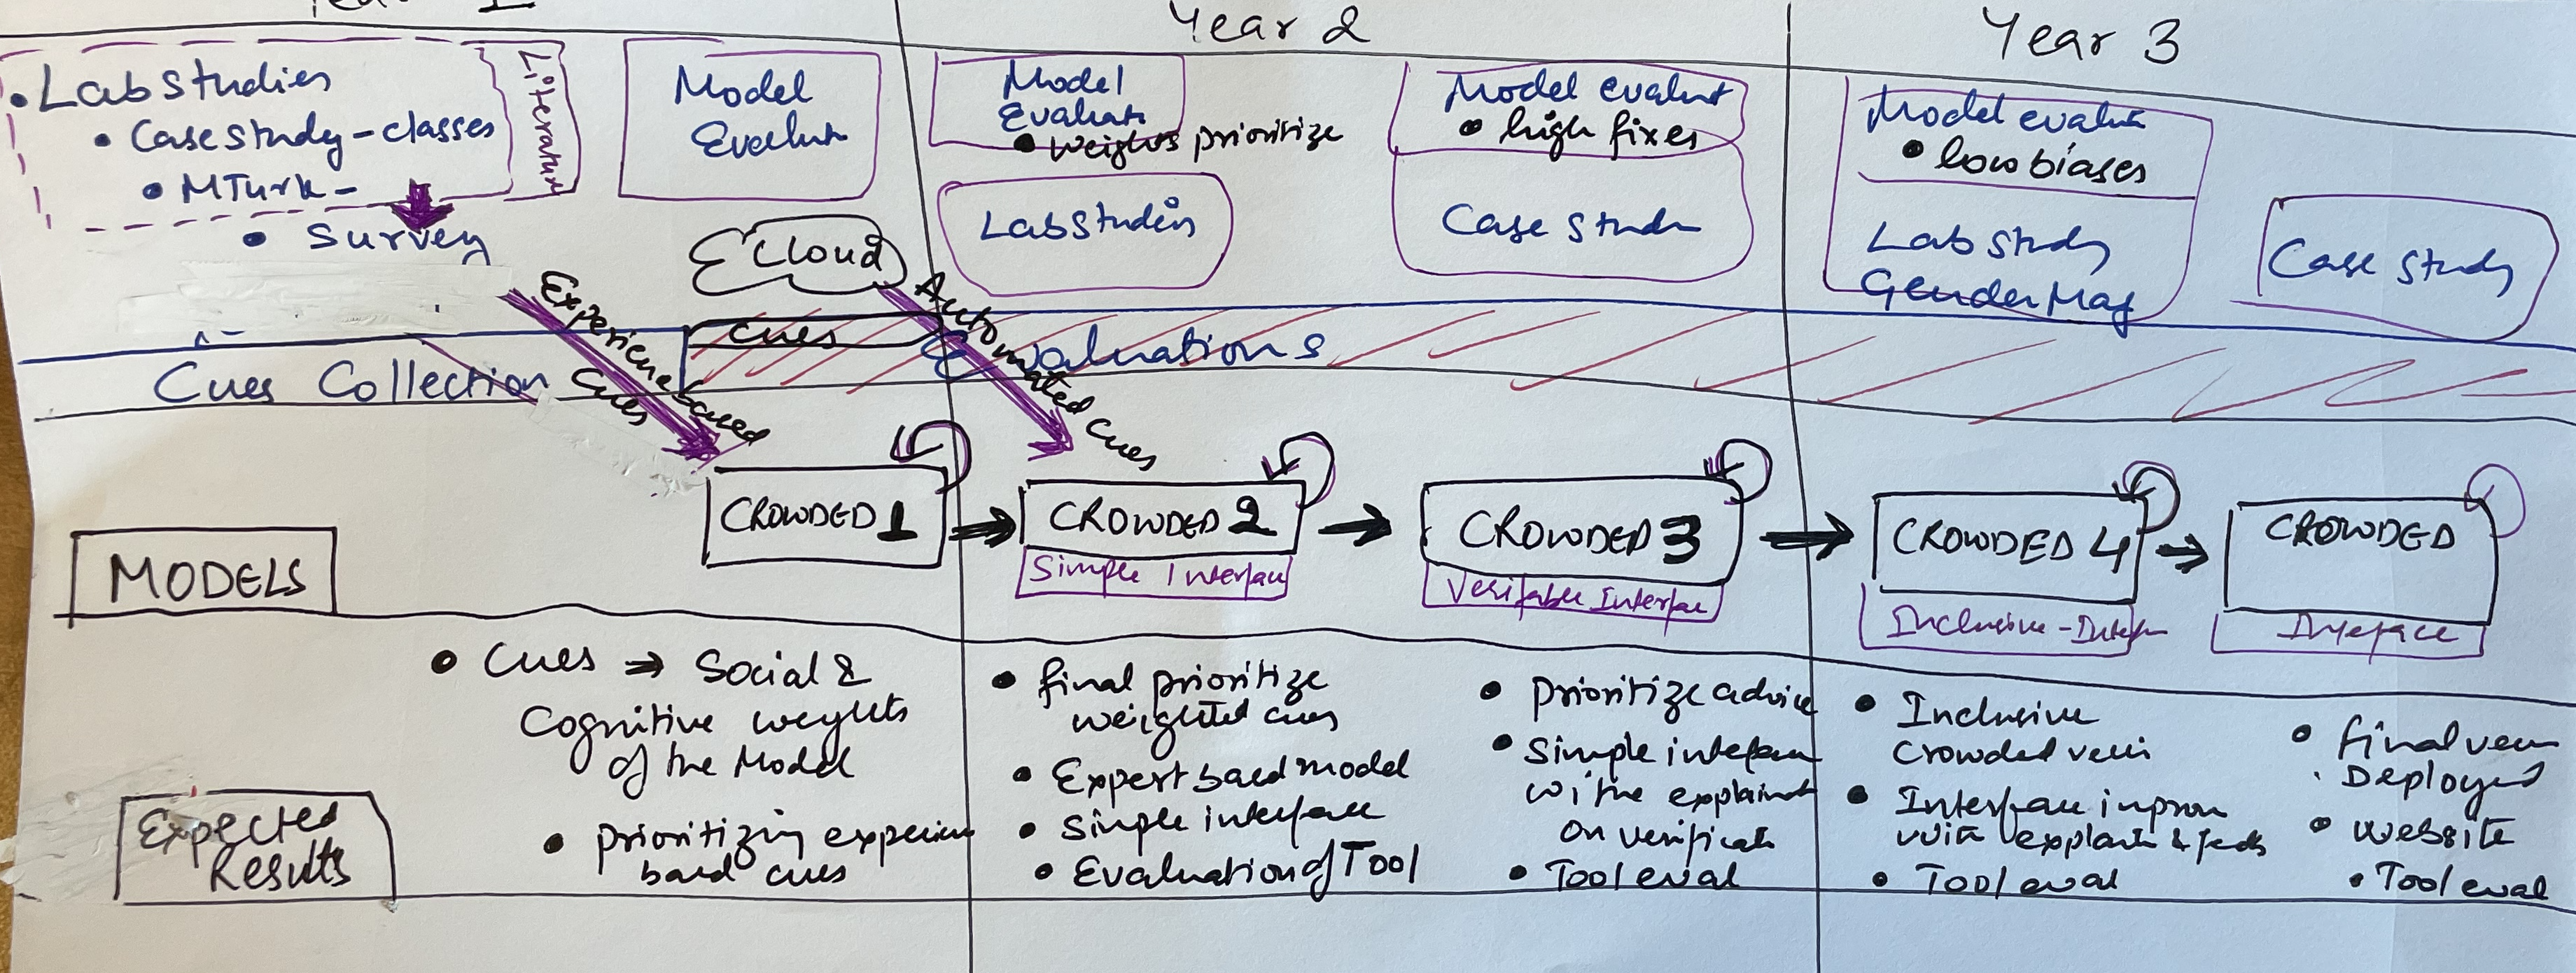
\includegraphics[width=0.98\textwidth]{fig/PLAN.PNG}}
% \caption{3-year plan. Initially our
% interface will be very simple (same as Fig6) bit as we learn more about the decision making styles needs of different classes of stakeholder's we will adjust our interface tools to give the explorations methods that suite their style.}
% \label{Overall}
% \end{figure*}


% \section{Overall Plan and Schedule}
% The proposed research will involve laboratory studies, interviews, surveys and case studies.  The continuous data collection, evaluation and refinement cycle will incrementally evolve ADVICE functionality. Figure \ref{Overall} shows the phased research plan over the three-year project period. 

% Efforts in Year 1 will focus on collecting Cues related to cognitive and social weights for ADVICE1-4 using ADVICE0. We will conduct gender and expert-balanced lab studies to collect initial set of cues utilized by the stakeholders when making decisions. Remember cues are the social and cognitive weights of the model that helps to prioritize the decision from different stakeholders. Further, to increase the reliability of the cues we will conduct case studies with students in SE classes and  professionals on Mturk. The tasks designed will help collect the respective cues as well as strategies when make decisions by stakeholders. Later, we will increase our confidence in the cues collected using lab study, case studies, and literature reviews by creating a large scale survey, followed by interviews. Towards end of Year1, the focus will be to develop ADVICE1 model that utilizes the expert's experience based cues and will be evaluated using model. RQ1 will be explored and user studies will measure: (i) higher accuracy of the model, and (ii) specific negation cliffs for the model weights. 

% In Year 2 the focus will be to develop ADVICE2 that utilizes cloud based cues (automatically generated from logs as in Table 2). We will evaluate the model with different weights to evaluate the best weight distribution strategy used by ADVICE2. Based on the finalized model we will use a simple interface to evaluate the model with gender and expert-balanced lab studies as well as case studies. We will collect qualitative and quantitative data.  Qualitative analyses will focus on transcripts and interviews; this will help also collect the decision style of different stakeholders. Quantitative analyses will employ the Wilcoxon rank-sum test or t-tests. The metrics include: (i) student and professional task success; (ii) completion times, (iii) student experiences (e.g., satisfaction and engagement) with ADVICE2 using end-of-term student course evaluations, (iv) accuracy of questionnare score with the model score. 

% Towards second half of Year2, ADVICE3 will be developed with verification support and will be evaluated by comparing various fixing techniques from literature for specific conflicts. ADVICE3 will be improved with better interface that generate feedback as well as explanations for ADVICE3 advice and decisions. ADVICE3 will evaluated using Comparative case studies with students and professionals. In class settings students will complete (i) first assignment without ADVICE3; (ii) second assignment with ADVICE3; and (iii) third assignment optionally with ADVICE3.  Similarly, using Mturk participants will complete decision making tasks with and without ADVICE3. Three-way ANOVA and two-way between-subjects tests will be used to measure decision performance and model acceptance. Further, the scores (from the model) will be compared to participants questionnaires. The results will also help assess the usability and generalizability of ADVICE3 in real-world settings. Additional metrics for model evaluation: Based on what we have seen in traditional software analytics, there are two expectations. (i) frequency of the Faulty advice, and (ii) time to fix faults (should have some exponential decay where most are fixed quickly, but a few may take comparatively much longer). We will explore RQ1-RQ6.

% In year3, we will develop ADVICE4, whose interface design will be inspired from gender-based research and evaluated with GenderMag (as discussed in Section XX). Further, the model will be improved to minimize social biases by including related measures in the PSO optimization goals.  Based on the finalized model we will evaluate ADVICE4 with gender and expert-balanced lab studies. We will collect qualitative and quantitative data.  Qualitative analyses will focus on transcripts and interviews. Quantitative analyses will employ the Wilcoxon rank-sum test or t-tests. Additional metrics: (i) gender-based biases, (ii) highest model accuracy with bias-based metrics. 

% The final version of ADVICE4 will be evaluated using case studies in the classes and using Mturk. We will collect the data from different race and gender especially in our MTurk studies.We will explore RQ1,R7-RQ11. 

%  A unique aspect of this project is that the research efforts will continuously advance educational initiatives that will constantly steer research activities to ensure that the results are robust, effective and practical.   During end of Year 3, the ADVICE prototype will also be disseminated to obtain feedback to continuously refining the prototype. ADVICE will support industry methods to advance decision making and, of course, increasing diversity in computer science .

% Lastly,  one  of the benefits of  NSF funding is the opportunity to work on  broadening participating in computing (BPC).  Our BPC plans are discussed in \S\ref{bpc}. As seen in our timetable, BPC will be an on-going task through-out the work.
  \section{Intellectual Merit and Broader Impact}
  

\subsection{Intellectual Merit}

%This research explores uncharted territories in SE, introducing innovative methodologies to address inference in the midst of team disputes. It distinguishes itself by prioritizing collective team decision-making and seamlessly integrating symbolic and sub-symbolic models, providing a multidimensional approach not present in current research paradigms. The transformative nature of this research promises to revolutionize decision-making in software design.
This research introduces methodologies in SE to address inference challenges during team disputes, navigating uncharted domains. In response to the surge in AI-assisted tools, a key innovation lies in actively incorporating human feedback, prioritizing collective team decision-making, and seamlessly integrating symbolic and sub-symbolic models. This multidimensional approach sets it apart from current research paradigms. The intellectual merits of this work encompass: (1) Methodological Framework: The development of a robust methodology applicable to decision-making domains, offering advancements for fellow researchers in diverse fields. (2) Model Sharing: Dissemination of models and the {\IT} tool to the wider research and practitioner communities, fostering collaboration and enhancing capabilities in software engineering and decision-making. (3) Algorithmic Insights: Contribution of valuable algorithms, visualizations, and essential decision-making parameters and rules, providing a foundational resource for informed choices and effective problem-solving. (4) Empirical Insights: Each study conducted to enhance {\IT} generates empirical data and insights, enriching the scientific understanding of decision-makers in the domain. This research has the potential to revolutionize software design decision-making.






%This research delves into unexplored domains of SE, introducing innovative methodologies addressing inference amidst team disputes.  The study distinguishes itself by prioritizing collective team decision-making and seamlessly integrating symbolic and sub-symbolic models, offering a rich, multidimensional approach absent in current research paradigms. Its transformative nature promises to revolutionize software design decision-making

%This research aims ro encompass the creation of an innovative and practical tool, ADVICE, designed to facilitate decision-making for first responders. Additionally, we make the following research contributions: (1) Methodological Framework: We have developed a robust methodology that can be readily applied by fellow researchers in related decision making domains, facilitating advancements in their work. 
%(2) Model Sharing: We are sharing our models and the ADVICE tool with the wider research and practitioner communities, fostering collaboration and enhancing the capabilities of professionals in software engineering and decision making fields. 
%(3) Algorithmic Insights: Our research contributes valuable algorithms, visualizations, and essential decision-making parameters and rules, providing a solid foundation for informed choices and problem-solving
%(4) Empirical Insights: Each study conducted to improve ADVICE generates empirical data and insights that contribute to the scientific understanding of the domain of decision makers.

\subsection{Broader Impacts}

The project's broader impact is comprehensive, addressing five crucial areas. (1) It advances discovery and enhances education by reshaping the curriculum for graduate Software Engineering classes. Engaged students delve into interdisciplinary research at the crossroads of AI, SE, and HCI. Additionally, they gain valuable hands-on experience through internships at NASA, fostering collaboration and the development of lifelong professional relationships. (2) The project is committed to actively mentoring underrepresented groups, reflecting the significant contributions of both PIs to diversity and inclusion. Students involved in the project will have the opportunity to attend prestigious events such as the Grace Hopper conference and the Richard Tapia Celebration of Diversity in Computing. Additionally, a dedicated portion of the grant will be allocated to support initiatives focused on Broadening Participation in Computing (BPC). (3) The collaboration with NASA enhances infrastructure, providing access to extensive logs and field data. The team's diverse expertise ensures robustness. (4) Broad dissemination will be achieved through  through the publication of research in leading SE venues and sharing knowledge via keynotes and invited talks. Emphasizing open science, all project scripts, models, and data will be accessible on GitHub, freely available for researchers and industrial practitioners. (5) The work explores the synergy between humans and AI, introducing transformative concepts in decision-making with applications in security, safety, and software engineering, thereby carrying significant societal implication

Further, the team is well-qualified and diverse, with members possessing the expertise needed for this research -  PI specializes in building AI optimizers and Co-PI excels in studying human subjects and creating tools tailored to their needs. Dr. Misty Davies, affiliated with NASA Ames and an expert in building fmtool models, is also part of the SMART-STEReO project. 








% Bringing humans in the loop of the decision-making process for AI-based systems is an important area to explore in SE research. This could help to mold models better to human processes and potentially make them more explainable or interpretable.
 
 %Given the rapid rise of AI-assisted tools for developers, exploring work that more closely involves human-feedback will be an important line of work, and one that bears fruit for various SE tasks.



 


	% \section{PI's strengths}
	
	% The proposed research will draw on Dr. Kuttal's experience creating human-centric tools for developers using user-centered design and evaluation approaches.  She have created tools that support programmer creativity \cite{Kuttal2020} and exploratory programming behavior \cite{Jernigan2017, Jernigan2015}, debugging web-based distributed programming \cite{KuttalSR13-chi, KuttalSR13, KuttalSBRKS19}, problem-solving techniques \cite{Jernigan2017, Jernigan2015}, gender-specific behavior \cite{Kuttal2021g, Kuttal2019, Alexposter2022}, socio-technical skills \cite{Abimposter2022,Abimgitposter2022,Diwanjiposter2022,Zhou2018, sarma2016hiring, KuttalCWBS21, KuttalSRW18, abs-1810-13062} and communication styles \cite{Kuttal2020}. She has also introduced theory for information seeking to three new domains including: 1) end-user developers debugging for visual web-based programs \cite{KuttalSR13, KuttalSBRKS19}, 2) developers foraging in the presence of variants of information (resulting in variations foraging theory) \cite{RagavanKHSPB16, RagavanPPHKSB17}, 3) variation foraging for end user programmers \cite{MartosKK16, KuttalKMB21, Kuttal13, KuttalSSR11, KuttalSRW18} and 4) developers foraging for socio-technical information on Stack Overflow and GitHub \cite{Abimposter2022,Abimgitposter2022,Diwanjiposter2022}. She is currently developing conversational agent for programmers \cite{Kuttal2020, Kuttal2021,tochipaper, RobeFSE2022, Robe2020, Hartposter2022, Alexposter2022}, supporting information foraging by utilizing agents’ collective foraging behavior \cite{Abimposter2022,Abimgitposter2022,Diwanjiposter2022}, and  studying developer's brain-to-brain interactions when problem-solving in same and mixed gender pairs.
	
	
%	Foraging enduser \cite{kuttal2013}, Visual resume \cite{sarma2016hiring}, technical and social \cite{Zhou2018}, problem solvings\cite{Jernigan2017, Jernigan2015} gender \cite{Kuttal2021g, Kuttal2019, Alexposter2022}